\documentclass{standalone}
\usepackage{xcolor}
\usepackage{tikz}
\usepackage{pgfplots}
\usetikzlibrary{calc}

\definecolor{pastelblue}{RGB}{160,210,255}
\definecolor{pastelpurple}{RGB}{200,180,255}

\begin{document}
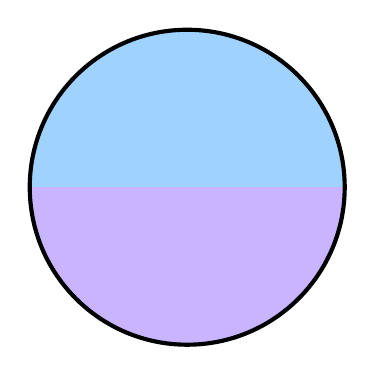
\begin{tikzpicture}
    % Pastel light blue semicircle with sum sign
    \fill [pastelblue] (0,2) arc (0:180:2) -- cycle;
	\fill [pastelpurple] (0,2) arc (0:-180:2) -- cycle;
    \draw[line width=1.5pt] (-2,2) circle (2);

% Pastel light blue semicircle with sum sign
%    \fill [pastelblue] (0,2) arc (90:270:2) -- cycle;
%    \node at (-1,0) {\resizebox{!}{2.7em}{\textcolor{black}{$\sum$}}};
    
    % Pastel light purple semicircle with ReLU function plot
%    \fill [pastelpurple] (0,2) arc (90:-90:2) -- cycle;
%    % ReLU function plot
%	\begin{axis}[hide axis, scale=0.2, shift={(50,-80)}]
%    	\addplot[domain=-2.:1.5, samples=100, black, line width=3.5pt] {max(0, x)};
%	\end{axis}

    % Circle outline with increased border thickness
%    \draw[line width=1.5pt] (0,0) circle (2);
      
\end{tikzpicture}
\end{document}